\section{The cylindrical detector system}

\begin{figure}[htbp]
  \centering
  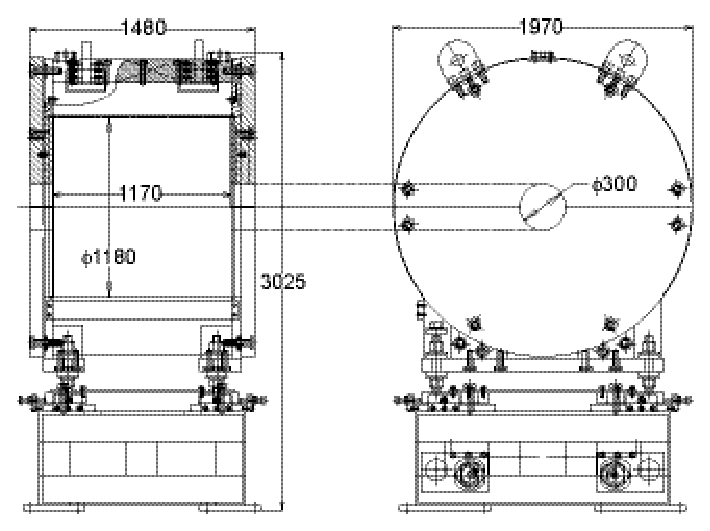
\includegraphics[width=8cm]{pic/experiment/solenoid.eps}
  \caption{
    Design of the solenoid magnet (all dimensions in mm)
  }
  \label{fig:CDS_solenoid}
\end{figure}
The cylindrical detector system (CDS) surrounds the experimental target system to measure produced charged particles.
The CDS consists of three parts, the outermost part is the solenoid magnet to make the uniform magnetic field for momentum analysis,
next is the cylindrical detector hodoscope (CDH) to measure time-of-flight from the T0 and make trigger signal,
and the cylindrical drift chamber (CDC) to measure the trajectory in the magnetic field, by which the momentum of a charged particle was analyzed. 
Particle identification was performed by the momentum and T0-CDH TOF.

\subsection{Solenoid magnet}
The CDS is a solenoid type spectrometer whose bore diameter is 1.18m and the length is 1.17m with an overall weight is about 23 tons.
The design of the solenoid magnet is shown in Fig\ref{fig:CDS_solenoid}.
The magnet provides a uniform field strength inside the tracking volume ($|z|<420mm$).
In the present experiment, it is operated at 0.7T.
